%%
%% This is file `sample-acmsmall-submission.tex',
%% generated with the docstrip utility.
%%
%% The original source files were:
%%
%% samples.dtx  (with options: `all,journal,bibtex,acmsmall-submission')
%%
%% IMPORTANT NOTICE:
%%
%% For the copyright see the source file.
%%
%% Any modified versions of this file must be renamed
%% with new filenames distinct from sample-acmsmall-submission.tex.
%%
%% For distribution of the original source see the terms
%% for copying and modification in the file samples.dtx.
%%
%% This generated file may be distributed as long as the
%% original source files, as listed above, are part of the
%% same distribution. (The sources need not necessarily be
%% in the same archive or directory.)
%%
%%
%% Commands for TeXCount
%TC:macro \cite [option:text,text]
%TC:macro \citep [option:text,text]
%TC:macro \citet [option:text,text]
%TC:envir table 0 1
%TC:envir table* 0 1
%TC:envir tabular [ignore] word
%TC:envir displaymath 0 word
%TC:envir math 0 word
%TC:envir comment 0 0
%%
%%
%% The first command in your LaTeX source must be the \documentclass
%% command.
%%
%% For submission and review of your manuscript please change the
%% command to \documentclass[manuscript, screen, review]{acmart}.
%%
%% When submitting camera ready or to TAPS, please change the command
%% to \documentclass[sigconf]{acmart} or whichever template is required
%% for your publication.
%%
%%
%\documentclass[acmsmall,screen,review]{acmart}
\documentclass[sigplan,anonymous,10pt]{acmart}
%\usepackage{listings}
\usepackage{url}
\usepackage{tlatex}
\usepackage{graphicx}
%\usepackage{tikz-uml}
\usepackage{color}
\definecolor{boxshade}{gray}{.95}
\setboolean{shading}{true}

%%
%% \BibTeX command to typeset BibTeX logo in the docs
\AtBeginDocument{%
  \providecommand\BibTeX{{%
    Bib\TeX}}}

%% Rights management information.  This information is sent to you
%% when you complete the rights form.  These commands have SAMPLE
%% values in them; it is your responsibility as an author to replace
%% the commands and values with those provided to you when you
%% complete the rights form.
\setcopyright{acmlicensed}
\copyrightyear{2024}
\acmYear{2024}
\acmDOI{XXXXXXX.XXXXXXX}

%%
%% These commands are for a JOURNAL article.
\acmJournal{JACM}
\acmVolume{37}
\acmNumber{4}
\acmArticle{111}
\acmMonth{8}

%%
%% Submission ID.
%% Use this when submitting an article to a sponsored event. You'll
%% receive a unique submission ID from the organizers
%% of the event, and this ID should be used as the parameter to this command.
%%\acmSubmissionID{123-A56-BU3}

%%
%% For managing citations, it is recommended to use bibliography
%% files in BibTeX format.
%%
%% You can then either use BibTeX with the ACM-Reference-Format style,
%% or BibLaTeX with the acmnumeric or acmauthoryear sytles, that include
%% support for advanced citation of software artefact from the
%% biblatex-software package, also separately available on CTAN.
%%
%% Look at the sample-*-biblatex.tex files for templates showcasing
%% the biblatex styles.
%%

%%
%% The majority of ACM publications use numbered citations and
%% references.  The command \citestyle{authoryear} switches to the
%% "author year" style.
%%
%% If you are preparing content for an event
%% sponsored by ACM SIGGRAPH, you must use the "author year" style of
%% citations and references.
%% Uncommenting
%% the next command will enable that style.
%%\citestyle{acmauthoryear}

%%
%% end of the preamble, start of the body of the document source.
\begin{document}

%%
%% The "title" command has an optional parameter,
%% allowing the author to define a "short title" to be used in page headers.
\title{Formal Verification of an RTOS Scheduler with TLA+}

%%
%% The "author" command and its associated commands are used to define
%% the authors and their affiliations.
%% Of note is the shared affiliation of the first two authors, and the
%% "authornote" and "authornotemark" commands
%% used to denote shared contribution to the research.
\author{J. German Rivera}
%\authornote{Both authors contributed equally to this research.}
\email{jgrivera67@gmail.com}
%\orcid{1234-5678-9012}
%\author{G.K.M. Tobin}
%\authornotemark[1]
%\email{webmaster@marysville-ohio.com}
\affiliation{%
  %\institution{Institute for Clarity in Documentation}
  \city{Austin}
  \state{Texas}
  \country{USA}
}

%%
%% The abstract is a short summary of the work to be presented in the
%% article.
\begin{abstract}
  This article describes an approach to do formal verification of the
  thread scheduler of a real-time operating system (RTOS) kernel via
  model checking. 
  The RTOS thread scheduler is modeled in TLA+/PlusCal at a level
  of abstraction close to actual code.
  The resulting model is checked with the TLA+ model checker (TLC),
  to verify that key safety invariants and liveness properties are
  satisfied by the thread scheduler.
  The RTOS being verified is \emph{HiRTOS} (\emph{High-Integrity}
  RTOS), a small RTOS kernel and separation kernel written in SPARK Ada.
  TLA+ is a mathematical modeling language for concurrent and distributed
  systems and PlusCal is a TLA+ companion procedural modeling language
  for specifying concurrent algorithms.
\end{abstract}

%%
%% The code below is generated by the tool at http://dl.acm.org/ccs.cfm.
%% Please copy and paste the code instead of the example below.
%%
\begin{CCSXML}
   <ccs2012>
      <concept>
          <concept_id>10011007</concept_id>
          <concept_desc>Software and its engineering</concept_desc>
          <concept_significance>500</concept_significance>
      </concept>
      <concept>
          <concept_id>10011007.10011074.10011099.10011692</concept_id>
          <concept_desc>Software and its engineering~Formal software verification</concept_desc>
          <concept_significance>500</concept_significance>
      </concept>
      <concept>
          <concept_id>10011007.10010940.10010941.10010949.10010957.10010688</concept_id>
          <concept_desc>Software and its engineering~Scheduling</concept_desc>
          <concept_significance>500</concept_significance>
      </concept>
   </ccs2012>
\end{CCSXML}
   
\ccsdesc[500]{Software and its engineering}
\ccsdesc[500]{Software and its engineering~Formal software verification}
\ccsdesc[500]{Software and its engineering~Scheduling}

%%
%% Keywords. The author(s) should pick words that accurately describe
%% the work being presented. Separate the keywords with commas.
\keywords{RTOS kernel, Thread Scheduler, Formal Verification, TLA+, Ada/SPARK}

\received{\today}
%\received[revised]{12 March 2009}
%\received[accepted]{5 June 2009}

%%
%% This command processes the author and affiliation and title
%% information and builds the first part of the formatted document.
\maketitle

\section{Introduction}

Doing formal verification of an RTOS thread scheduler can be challenging
due to the concurrent execution of multiple control flows. An RTOS
controls the interleaved execution of multiple threads.
The thread scheduler can be invoked synchronously or asynchronously
with respect to the current thread. The synchronous case is when
the thread scheduler is invoked as a result of the current thread
invoking an RTOS synchronization primitive, such as acquiring or
releasing a mutex.
The asynchronous case is when the scheduler is invoked on the return
path of an interrupt service routine (ISR), as part of the mechanism
to implement thread preemption.

Using a model checker for concurrent systems can be a way of doing
formal verification of an RTOS thread scheduler. To do this, first,
we need to create a model of the thread scheduler in the input language
of the model checker. Then, we run the model checker on the created model
to verify if it satisfies a set of correctness properties (safety invariants
and liveness properties). The model checker generates all possible
``interleavings'' of steps of the concurrent entities (threads and ISRs)
represented in the model. At every step, the model checker checks if the
correctness properties being verified hold. If a property is violated,
that means that the model checker has found a ``counter-example'' for the
property, which may indicate that there is design defect in the thread
scheduler or the model itself is wrong, or the property has something 
wrong.
As an example of this approach for doing formal verification of an RTOS
thread scheduler, this article describes how the HiRTOS thread scheduler
was modeled in TLA+/PlusCal and formally verified using the TLA+ model 
checker (TLC). 

HiRTOS (\emph{High Integrity} RTOS) \cite{HiRTOS} is a small RTOS 
kernel and separation kernel for embedded single-core and multi-core 
platforms that have a memory protection unit (MPU).
HiRTOS has a preemptive thread scheduler with fixed priorities and
round-robin for threads with the same priority.
On a multi-core platform, each core has its own thread scheduler and threads
always execute in the same core where they were created. No HiRTOS resources
are shared between CPUs and no communication/synchronization across CPU
cores is supported by HiRTOS. Mutexes and condition variables \cite{mutexAndCV}
are the only synchronization primitives in HiRTOS, and they only support
synchronizing threads running on the same core. HiRTOS mutexes support both
priority inheritance and priority ceiling protocols \cite{prioCeiling}.
Unlike traditional condition variables, HiRTOS condition variables
can also be waited on while having interrupts disabled, not just while holding
a mutex.

Given the fact that there is a separate instance of the HiRTOS scheduler per CPU,
and there is no interaction between CPUs at the HiRTOS level, we just need to do
formal verification of the HiRTOS thread scheduler for the single-core case.

HiRTOS is written in the SPARK subset of Ada \cite{SparkAda}, without using pointers (Ada access types).
All RTOS objects such as threads, mutexes and condition variables are allocated internally
by HiRTOS, from statically allocated internal object pools. 
These object pools are RTOS-private global arrays of the corresponding RTOS object types,
sized at compile time via configuration parameters, whose values are application-specific.
RTOS object handles provided to application code are just indices into these internal object arrays.
No actual RTOS object pointers are exposed to application code.
No dynamic allocation/deallocation of RTOS objects is supported and no static allocation of RTOS
objects in memory owned by application code is supported either.

Since HiRTOS is implemented in SPARK Ada, its code can be formally verified, up to some
degree, using the \verb'gnatprove' tool \cite{gnatprove}. For example, absence of Ada
runtime errors can be formally verified with \verb'gnatprove', as well as pre/post-condition
contracts of individual subprograms. However, overall safety invariants and liveness
properties of the concurrent execution flows in HiRTOS cannot be verified with
\verb'gnatprove'. We need to use another kind of formal verification tool.
A suitable tool is the TLA+ model checker (TLC) \cite{tlc}.
TLA+ \cite{tla1}, which
stands for ``Temporal Logic of Actions'', is a mathematical modeling language for concurrent
and distributed systems, based on set theory, predicate logic and temporal logic.
PlusCal \cite{PlusCal,tla2} is
a TLA+ companion language for specifying/modeling concurrent and distributed algorithms.
A PlusCal model is ``compiled'' to a TLA+ model, which can be checked with TLC. 

The rest of this paper is organized as follows. Section 2 describes the invocation points
of the HiRTOS thread scheduler.
Section 3 presents a TLA+ model of the HiRTOS per-cpu internal data structures.
Section 4 presents the PlusCal model of the HiRTOS thread scheduler.
Section 5 presents the safety invariants and liveness properties that were checked.
The complete TLA+/PlusCal model can be
found in the HiRTOS GitHub repository at \url{https://github.com/jgrivera67/HiRTOS/blob/main/doc/tla_model/HiRTOS.tla}.

\section{HiRTOS Thread Scheduler Overview}

\subsection{Initial Invocation of the Thread Scheduler}

The HIRTOS thread scheduler is first invoked at boot-time, when the application code's
reset handler calls The HIRTOS primitive to start the scheduler. This primitive,
instead of returning to the caller, executes the logic to return from an interrupt,
which causes the highest priority thread to be switched-in.

\subsection{Asynchronous Invocation of the Thread Scheduler}

In HiRTOS, thread preemption is implemented by invoking the thread scheduler
on the exit path of an interrupt handler. When an interrupt fires while
a thread is running, the executing thread's CPU context is saved
on thread's stack by the interrupt handler prolog. Then, before calling the
actual interrupt handler, the stack is switched to the interrupt handling stack.
After the interrupt handler returns, the interrupt handler epilog invokes
the HiRTOS thread scheduler, to select the highest priority runnable thread.
Then, if the newly selected thread is different from  the one that was running before
the interrupt, the extended context of the old thread is saved and the extended
context of the new thread is restored.

\subsection{Synchronous Invocation of the Thread Scheduler}

In HiRTOS, the thread scheduler is invoked synchronously from a thread
in the following cases:

\begin{itemize}
\item When a thread calls \verb`HiRTOS.Condvar.Wait`
\item When a thread calls \verb`HiRTOS.Condvar.Signal` 
      and there are threads waiting on the condition variable
\item When a thread calls \verb`HiRTOS.Condvar.Broadcast`
      and there are threads waiting on the condition variable     
\item When a thread calls \verb`HiRTOS.Mutex.Acquire` and the mutex is not available
\item When a thread calls \verb`HiRTOs.Mutex.Release` and there are threads waiting
      to acquire the mutex
\item When a thread calls \verb`HiRTOS.Thread.Thread_Delay_Until`, which in turn calls
      \verb`HiRTOS.Condvar.Wait` for the thread's builtin condition variable.
\item When a thread calls \verb`HiRTOS.Thread.Suspend_Current_Thread`
\item When a thread calls \verb`HiRTOS.Thread.Resume_Thread`
\item When a thread calls \verb`HiRTOS.Restore_Atomic_Level` and the old atomic level is
      \verb`Atomic_Level_None`
\end{itemize}

\section{TLA+/PlusCal Model of HiRTOS Per-CPU Internal Data Structures}

\subsection{PlusCal Model of HiRTOS Per-CPU Global State}

The per-CPU global state of HiRTOS is modeled by the following PlusCal
global variables, initialized for a specific scenario with three application
threads: 
\begin{ppcal}
HiRTOS = [
   Current_Thread_Id |-> "Invalid_Thread_Id",
   Runnable_Threads_Queue |->
        [ p \in Valid_Thread_Priority_Type |->
            CASE p = 0 -> <<"Idle_Thread">>
            [] p = 1 -> <<"thread1">>
            [] p = 2 -> <<"thread2", "thread3">>
        ],
   Interrupts_Enabled |-> FALSE
],
Thread_Objects = [
   Idle_Thread |->
      Thread_Object_Initializer(0, "Invalid_Timer_Id", 
                                "Invalid_Condvar_Id"),
   thread1 |->
      Thread_Object_Initializer(1, "thread1_timer", 
                                "thread1_condvar"),
   thread2 |->
      Thread_Object_Initializer(2, "thread2_timer", 
                                "thread2_condvar"),
   thread3 |->
      Thread_Object_Initializer(2, "thread3_timer",
                                "thread3_condvar")
],
Mutex_Objects = 
   [ m \in Mutexes |-> Mutex_Object_Initializer ],
Condvar_Objects =
   [ cv \in Condvars |-> Condvar_Object_Initializer ],
Timer_Objects =
   [ tm \in Timers |-> Timer_Object_Initializer ],
Global_Resource_Available = FALSE;
\end{ppcal}
\begin{tlatex}
\@x{ HiRTOS \.{=} [}%
\@x{\@s{12.29} Current\_Thread\_Id \.{\mapsto}\@w{Invalid\_Thread\_Id} ,\,}%
\@x{\@s{12.29} Runnable\_Threads\_Queue \.{\mapsto}}%
\@x{\@s{32.8} [ p \.{\in} Valid\_Thread\_Priority\_Type \.{\mapsto}}%
 \@x{\@s{42.77} {\CASE} p \.{=} 0 \.{\rightarrow} {\langle}\@w{Idle\_Thread}
 {\rangle}}%
 \@x{\@s{42.77} {\Box} p \.{=} 1 \.{\rightarrow} {\langle}\@w{thread1}
 {\rangle}}%
 \@x{\@s{42.77} {\Box} p \.{=} 2 \.{\rightarrow} {\langle}\@w{thread2}
 ,\,\@w{thread3} {\rangle}}%
\@x{\@s{32.8} ] ,\,}%
\@x{\@s{12.29} Interrupts\_Enabled \.{\mapsto} {\FALSE}}%
\@x{ ] ,\,}%
\@x{ Thread\_Objects \.{=} [}%
\@x{\@s{12.29} Idle\_Thread \.{\mapsto}}%
 \@x{\@s{24.59} Thread\_Object\_Initializer ( 0 ,\,\@w{Invalid\_Timer\_Id}
 ,\,}%
\@x{\@s{141.06}\@w{Invalid\_Condvar\_Id} ) ,\,}%
\@x{\@s{12.29} thread1 \.{\mapsto}}%
\@x{\@s{24.59} Thread\_Object\_Initializer ( 1 ,\,\@w{thread1\_timer} ,\,}%
\@x{\@s{141.06}\@w{thread1\_condvar} ) ,\,}%
\@x{\@s{12.29} thread2 \.{\mapsto}}%
\@x{\@s{24.59} Thread\_Object\_Initializer ( 2 ,\,\@w{thread2\_timer} ,\,}%
\@x{\@s{141.06}\@w{thread2\_condvar} ) ,\,}%
\@x{\@s{12.29} thread3 \.{\mapsto}}%
\@x{\@s{24.59} Thread\_Object\_Initializer ( 2 ,\,\@w{thread3\_timer} ,\,}%
\@x{\@s{141.06}\@w{thread3\_condvar} )}%
\@x{ ] ,\,}%
\@x{ Mutex\_Objects \.{=}}%
 \@x{\@s{12.29} [ m \.{\in} Mutexes \.{\mapsto} Mutex\_Object\_Initializer ]
 ,\,}%
\@x{ Condvar\_Objects \.{=}}%
 \@x{\@s{12.29} [ cv \.{\in} Condvars \.{\mapsto} Condvar\_Object\_Initializer
 ] ,\,}%
\@x{ Timer\_Objects \.{=}}%
 \@x{\@s{12.29} [ tm \.{\in} Timers \.{\mapsto} Timer\_Object\_Initializer ]
 ,\,}%
\@x{ Global\_Resource\_Available \.{=} {\FALSE} {\p@semicolon}}%
\end{tlatex}

\subsection{TLA+ Model of a HiRTOS Thread Control Block}
\begin{tla}
Thread_Object_Type == [
    State : Thread_State_Type,
    Current_Priority : Valid_Thread_Priority_Type,
    Base_Priority : Valid_Thread_Priority_Type,
    Builtin_Timer_Id : Timer_Id_Type,
    Builtin_Condvar_Id : Condvar_Id_Type,
    Waiting_On_Condvar_Id : Condvar_Id_Type,
    Waiting_On_Mutex_Id : Mutex_Id_Type,
    Owned_Mutexes : 
      Injective_Sequence_Type(Mutex_Id_Type),
    ghost_Time_Slice_Consumed : BOOLEAN,
    ghost_Condvar_Wait_Mutex_Id : Mutex_Id_Type
]

Thread_Object_Initializer(priority, timer_id, 
                          condvar_id) == [
    State |-> "Runnable",
    Current_Priority |-> priority,
    Base_Priority  |-> priority,
    Builtin_Timer_Id |-> timer_id,
    Builtin_Condvar_Id |-> condvar_id,
    Waiting_On_Condvar_Id |-> "Invalid_Condvar_Id",
    Waiting_On_Mutex_Id |-> "Invalid_Mutex_Id",
    Owned_Mutexes |-> <<>>,
    Time_Slice_Consumed |-> FALSE,
    Condvar_Wait_Mutex_Id |-> "Invalid_Mutex_Id"
]
\end{tla}
\begin{tlatex}
\@x{ Thread\_Object\_Type \.{\defeq} [}%
\@x{\@s{16.4} State \.{:} Thread\_State\_Type ,\,}%
\@x{\@s{16.4} Current\_Priority \.{:} Valid\_Thread\_Priority\_Type ,\,}%
\@x{\@s{16.4} Base\_Priority \.{:} Valid\_Thread\_Priority\_Type ,\,}%
\@x{\@s{16.4} Builtin\_Timer\_Id \.{:} Timer\_Id\_Type ,\,}%
\@x{\@s{16.4} Builtin\_Condvar\_Id \.{:} Condvar\_Id\_Type ,\,}%
\@x{\@s{16.4} Waiting\_On\_Condvar\_Id \.{:} Condvar\_Id\_Type ,\,}%
\@x{\@s{16.4} Waiting\_On\_Mutex\_Id \.{:} Mutex\_Id\_Type ,\,}%
\@x{\@s{16.4} Owned\_Mutexes \.{:}}%
\@x{\@s{24.59} Injective\_Sequence\_Type ( Mutex\_Id\_Type ) ,\,}%
\@x{\@s{16.4} ghost\_Time\_Slice\_Consumed \.{:} {\BOOLEAN} ,\,}%
\@x{\@s{16.4} ghost\_Condvar\_Wait\_Mutex\_Id \.{:} Mutex\_Id\_Type}%
\@x{ ]}%
\@pvspace{8.0pt}%
\@x{ Thread\_Object\_Initializer ( priority ,\, timer\_id ,\,}%
\@x{\@s{116.46} condvar\_id ) \.{\defeq} [}%
\@x{\@s{16.4} State \.{\mapsto}\@w{Runnable} ,\,}%
\@x{\@s{16.4} Current\_Priority \.{\mapsto} priority ,\,}%
\@x{\@s{16.4} Base\_Priority\@s{4.1} \.{\mapsto} priority ,\,}%
\@x{\@s{16.4} Builtin\_Timer\_Id \.{\mapsto} timer\_id ,\,}%
\@x{\@s{16.4} Builtin\_Condvar\_Id \.{\mapsto} condvar\_id ,\,}%
 \@x{\@s{16.4} Waiting\_On\_Condvar\_Id \.{\mapsto}\@w{Invalid\_Condvar\_Id}
 ,\,}%
\@x{\@s{16.4} Waiting\_On\_Mutex\_Id \.{\mapsto}\@w{Invalid\_Mutex\_Id} ,\,}%
\@x{\@s{16.4} Owned\_Mutexes \.{\mapsto} {\langle} {\rangle} ,\,}%
\@x{\@s{16.4} Time\_Slice\_Consumed \.{\mapsto} {\FALSE} ,\,}%
\@x{\@s{16.4} Condvar\_Wait\_Mutex\_Id \.{\mapsto}\@w{Invalid\_Mutex\_Id}}%
\@x{ ]}%
\end{tlatex}

\subsection{TLA+ Model of a HiRTOS Mutex Object}
\begin{tla}
Mutex_Object_Type == [
    Owner_Thread_Id : Thread_Id_Type,
    Last_Inherited_Priority : Thread_Priority_Type,
    Waiting_Threads_Queue : 
      Thread_Priority_Queue_Type
]

Mutex_Object_Initializer == [
    Owner_Thread_Id |-> "Invalid_Thread_Id",
    Last_Inherited_Priority |-> Invalid_Thread_Priority,
    Waiting_Threads_Queue |->
        [ p \in Valid_Thread_Priority_Type |-> <<>> ]
]
\end{tla}
\begin{tlatex}
\@x{ Mutex\_Object\_Type \.{\defeq} [}%
\@x{\@s{16.4} Owner\_Thread\_Id \.{:} Thread\_Id\_Type ,\,}%
\@x{\@s{16.4} Last\_Inherited\_Priority \.{:} Thread\_Priority\_Type ,\,}%
\@x{\@s{16.4} Waiting\_Threads\_Queue \.{:}}%
\@x{\@s{24.59} Thread\_Priority\_Queue\_Type}%
\@x{ ]}%
\@pvspace{8.0pt}%
\@x{ Mutex\_Object\_Initializer \.{\defeq} [}%
\@x{\@s{16.4} Owner\_Thread\_Id \.{\mapsto}\@w{Invalid\_Thread\_Id} ,\,}%
 \@x{\@s{16.4} Last\_Inherited\_Priority \.{\mapsto} Invalid\_Thread\_Priority
 ,\,}%
\@x{\@s{16.4} Waiting\_Threads\_Queue \.{\mapsto}}%
 \@x{\@s{32.8} [ p \.{\in} Valid\_Thread\_Priority\_Type \.{\mapsto} {\langle}
 {\rangle} ]}%
\@x{ ]}%
\end{tlatex}

\subsection{TLA+ Model of a HiRTOS Condition Variable Object}
\begin{tla}
Condvar_Object_Type == [
    Wakeup_Mutex_Id : Mutex_Id_Type,
    Waiting_Threads_Queue : 
      Thread_Priority_Queue_Type
]

Condvar_Object_Initializer == [
    Wakeup_Mutex_Id |-> "Invalid_Mutex_Id",
    Waiting_Threads_Queue |->
        [ p \in Valid_Thread_Priority_Type |-> <<>> ]
]
\end{tla}
\begin{tlatex}
\@x{ Condvar\_Object\_Type \.{\defeq} [}%
\@x{\@s{16.4} Wakeup\_Mutex\_Id \.{:} Mutex\_Id\_Type ,\,}%
\@x{\@s{16.4} Waiting\_Threads\_Queue \.{:}}%
\@x{\@s{24.59} Thread\_Priority\_Queue\_Type}%
\@x{ ]}%
\@pvspace{8.0pt}%
\@x{ Condvar\_Object\_Initializer \.{\defeq} [}%
\@x{\@s{16.4} Wakeup\_Mutex\_Id \.{\mapsto}\@w{Invalid\_Mutex\_Id} ,\,}%
\@x{\@s{16.4} Waiting\_Threads\_Queue \.{\mapsto}}%
 \@x{\@s{32.8} [ p \.{\in} Valid\_Thread\_Priority\_Type \.{\mapsto} {\langle}
 {\rangle} ]}%
\@x{ ]}%
\end{tlatex}

\section{PlusCal Model of HiRTOS Control Flows}

HiRTOS concurrent control flows are modeled as PlusCal
processes.
% A PlusCal process consists of a sequence
% of atomic steps. Each atomic step is tagged with a label and 
% consists of one or more PlusCal action statements, such as 
% assignments, \verb'await' and \verb'skip'. \verb`await` blocks
% the execution of the process until a condition becomes true.
% In addition to action statements, a process can also have 
% control flow statements such as \verb`if/else` conditionals,
% \verb`while` loops, \verb`either` non-deterministic blocks 
% and procedure calls.

\subsection{Reset Handler}
\begin{ppcal}
fair process Reset_Handler = "Reset_Handler"
begin
   cpu_starts:
   \* *** Boot-time initializations before RTOS tasking is turned on: ***
   skip;

   \* *** Turn on RTOS tasking: ***
   start_scheduler:
   call Run_Thread_Scheduler();
   scheduler_started:
   HiRTOS.Interrupts_Enabled := TRUE;
end process;
\end{ppcal}
\begin{tlatex}
\@x{ {\p@fair} {\p@process} Reset\_Handler \.{=}\@w{Reset\_Handler}}%
\@x{ {\p@begin}}%
\@x{\@s{12.29} cpu\_starts\@s{.5}\textrm{:}\@s{3}}%
\@x{\@s{12.29}}%
\@y{%
  *** Boot-time initializations before RTOS tasking is turned on: ***
}%
\@xx{}%
\@x{\@s{12.29} {\p@skip} {\p@semicolon}}%
\@pvspace{8.0pt}%
\@x{\@s{12.29}}%
\@y{%
  *** Turn on RTOS tasking: ***
}%
\@xx{}%
\@x{\@s{12.29} start\_scheduler\@s{.5}\textrm{:}\@s{3}}%
\@x{\@s{12.29} {\p@call} Run\_Thread\_Scheduler ( ) {\p@semicolon}}%
\@x{\@s{12.29} scheduler\_started\@s{.5}\textrm{:}\@s{3}}%
\@x{\@s{12.29} HiRTOS . Interrupts\_Enabled \.{:=} {\TRUE} {\p@semicolon}}%
\@x{ {\p@end} {\p@process} {\p@semicolon}}%
\end{tlatex}

% At boot time, the CPU starts executing instructions at the reset handler
% entry point.
The reset handler or the application main (invoked from the reset handler)
calls the HiRTOS API to start the scheduler.
This API never returns. Instead, it makes the reset handler exit, like if
it were an ISR exiting.
No threads or interrupts can execute before the HiRTOS
thread scheduler is started. 
This is modeled in PlusCal by making the \verb`Reset_Handler`
process, the only executable process initially, as interrupts are disabled
initially. 

\subsection{Application Threads}

\begin{ppcal}
fair process App_Thread \in Threads \ { "Idle_Thread" }
begin
   thread_state_machine_next_state_loop:
   while TRUE do
      \* *** Thread context switch happens here: ***
      await Thread_Objects[self].State = "Running" /\ 
            HiRTOS.Interrupts_Enabled;
      either
         acquire_mutex_step:
         call Acquire_Mutex("mutex1");

         either_wait_or_skip_step:
         either
             waiting_for_resource_step:
             while ~Global_Resource_Available do
                 call Wait_On_Condvar("condvar1",
                                      "mutex1");
             end while;

             Global_Resource_Available := FALSE;
         or
           skip;
         end either;

         release_mutex_step:
         call Release_Mutex("mutex1");
      or
         Global_Resource_Available := TRUE;
         either
            call Signal_Condvar("condvar1");
         or
            call Broadcast_Condvar("condvar1");
         end either;
      or
         call Delay_Until()
       end either;

      thread_iteration_completed_step:
      skip;
   end while;
end process;
\end{ppcal}
\begin{tlatex}
 \@x{ {\p@fair} {\p@process} App\_Thread \.{\in} Threads \.{\,\backslash\,}
 \{\@w{Idle\_Thread} \}}%
\@x{ {\p@begin}}%
\@x{\@s{12.29} thread\_state\_machine\_next\_state\_loop\@s{.5}\textrm{:}\@s{3}}%
\@x{\@s{12.29} {\p@while} {\TRUE} {\p@do}}%
\@x{\@s{24.59}}%
\@y{%
  *** Thread context switch happens here: ***
}%
\@xx{}%
 \@x{\@s{24.59} {\p@await} Thread\_Objects [ self ] . State \.{=}\@w{Running}
 \.{\land}}%
\@x{\@s{51.78} HiRTOS . Interrupts\_Enabled {\p@semicolon}}%
\@x{\@s{24.59} {\p@either}}%
\@x{\@s{36.89} acquire\_mutex\_step\@s{.5}\textrm{:}\@s{3}}%
\@x{\@s{36.89} {\p@call} Acquire\_Mutex (\@w{mutex1} ) {\p@semicolon}}%
\@pvspace{8.0pt}%
\@x{\@s{36.89} either\_wait\_or\_skip\_step\@s{.5}\textrm{:}\@s{3}}%
\@x{\@s{36.89} {\p@either}}%
\@x{\@s{53.29} waiting\_for\_resource\_step\@s{.5}\textrm{:}\@s{3}}%
\@x{\@s{53.29} {\p@while} {\lnot} Global\_Resource\_Available {\p@do}}%
\@x{\@s{69.7} {\p@call} Wait\_On\_Condvar (\@w{condvar1} ,\,}%
\@x{\@s{175.26}\@w{mutex1} ) {\p@semicolon}}%
\@x{\@s{53.29} {\p@end} {\p@while} {\p@semicolon}}%
\@pvspace{8.0pt}%
\@x{\@s{53.29} Global\_Resource\_Available \.{:=} {\FALSE} {\p@semicolon}}%
\@x{\@s{36.89} {\p@or}}%
\@x{\@s{45.1} {\p@skip} {\p@semicolon}}%
\@x{\@s{36.89} {\p@end} {\p@either} {\p@semicolon}}%
\@pvspace{8.0pt}%
\@x{\@s{36.89} release\_mutex\_step\@s{.5}\textrm{:}\@s{3}}%
\@x{\@s{36.89} {\p@call} Release\_Mutex (\@w{mutex1} ) {\p@semicolon}}%
\@x{\@s{24.59} {\p@or}}%
\@x{\@s{36.89} Global\_Resource\_Available \.{:=} {\TRUE} {\p@semicolon}}%
\@x{\@s{36.89} {\p@either}}%
\@x{\@s{49.19} {\p@call} Signal\_Condvar (\@w{condvar1} ) {\p@semicolon}}%
\@x{\@s{36.89} {\p@or}}%
\@x{\@s{49.19} {\p@call} Broadcast\_Condvar (\@w{condvar1} ) {\p@semicolon}}%
\@x{\@s{36.89} {\p@end} {\p@either} {\p@semicolon}}%
\@x{\@s{24.59} {\p@or}}%
\@x{\@s{36.89} {\p@call} Delay\_Until ( )}%
\@x{\@s{28.69} {\p@end} {\p@either} {\p@semicolon}}%
\@pvspace{8.0pt}%
\@x{\@s{24.59} thread\_iteration\_completed\_step\@s{.5}\textrm{:}\@s{3}}%
\@x{\@s{24.59} {\p@skip} {\p@semicolon}}%
\@x{\@s{12.29} {\p@end} {\p@while} {\p@semicolon}}%
\@x{ {\p@end} {\p@process} {\p@semicolon}}%
\end{tlatex}

There is one \verb`App_Thread` process for each application thread.

\subsection{Idle Thread}
\begin{ppcal}
fair process Idle_Thread = "Idle_Thread"
begin
   idle_thread_next_state_loop:
   while TRUE do
       await Thread_Objects["Idle_Thread"].State = 
                "Running" /\
             HiRTOS.Interrupts_Enabled;
   end while;
end process;
\end{ppcal}
\begin{tlatex}
\@x{ {\p@fair} {\p@process} Idle\_Thread \.{=}\@w{Idle\_Thread}}%
\@x{ {\p@begin}}%
\@x{\@s{12.29} idle\_thread\_next\_state\_loop\@s{.5}\textrm{:}\@s{3}}%
\@x{\@s{12.29} {\p@while} {\TRUE} {\p@do}}%
\@x{\@s{28.69} {\p@await} Thread\_Objects [\@w{Idle\_Thread} ] . State \.{=}}%
\@x{\@s{68.18}\@w{Running} \.{\land}}%
\@x{\@s{55.88} HiRTOS . Interrupts\_Enabled {\p@semicolon}}%
\@x{\@s{12.29} {\p@end} {\p@while} {\p@semicolon}}%
\@x{ {\p@end} {\p@process} {\p@semicolon}}%
\end{tlatex}

\subsection{Timer Interrupt Handler}
\begin{ppcal}
fair process Timer_Interrupt = "Timer_Interrupt"
   variable delayed_threads = {};
begin
   timer_interrupt_next_state_loop:
   while TRUE do
      enter_critical_section_step:
      Enter_Critical_Section("Timer_Interrupt");

      track_time_slice:
      if HiRTOS.Current_Thread_Id /= "Invalid_Thread_Id" 
      then
         assert ~Thread_Objects[
                    HiRTOS.Current_Thread_Id].
                       Time_Slice_Consumed;
         Thread_Objects[HiRTOS.Current_Thread_Id].
            Time_Slice_Consumed := TRUE;
      end if;

      delayed_threads :=
         { t \in Threads \ { "Idle_Thread" } :
           Timer_Objects[
              Thread_Objects[t].Builtin_Timer_Id].
                 State = "Timer_Running" };

      wakeup_delay_until_waiters:
      while delayed_threads /= {} do
         with t \in delayed_threads do
            delayed_threads := delayed_threads \ {t};
            Timer_Objects[Thread_Objects[t].
               Builtin_Timer_Id].State := "Timer_Stopped";
            call Do_Signal_Condvar(
                   Thread_Objects[t].Builtin_Condvar_Id,
                   FALSE);
          end with;
      end while;

      \* *** Thread scheduler invoked when exiting the ISR: ***
      timer_interupt_asynchronous_context_switch_step:
      call Run_Thread_Scheduler();

      exit_critical_section_step:
      Exit_Critical_Section();
   end while;
end process;
\end{ppcal}
\begin{tlatex}
\@x{ {\p@fair} {\p@process} Timer\_Interrupt \.{=}\@w{Timer\_Interrupt}}%
\@x{\@s{12.29} {\p@variable} delayed\_threads \.{=} \{ \} {\p@semicolon}}%
\@x{ {\p@begin}}%
\@x{\@s{12.29} timer\_interrupt\_next\_state\_loop\@s{.5}\textrm{:}\@s{3}}%
\@x{\@s{12.29} {\p@while} {\TRUE} {\p@do}}%
\@x{\@s{24.59} enter\_critical\_section\_step\@s{.5}\textrm{:}\@s{3}}%
 \@x{\@s{24.59} Enter\_Critical\_Section (\@w{Timer\_Interrupt} )
 {\p@semicolon}}%
\@pvspace{8.0pt}%
\@x{\@s{24.59} track\_time\_slice\@s{.5}\textrm{:}\@s{3}}%
 \@x{\@s{24.59} {\p@if} HiRTOS . Current\_Thread\_Id
 \.{\neq}\@w{Invalid\_Thread\_Id}}%
\@x{\@s{24.59} {\p@then}}%
\@x{\@s{36.89} {\p@assert} {\lnot} Thread\_Objects [}%
\@x{\@s{84.44} HiRTOS . Current\_Thread\_Id ] .}%
\@x{\@s{96.74} Time\_Slice\_Consumed {\p@semicolon}}%
\@x{\@s{36.89} Thread\_Objects [ HiRTOS . Current\_Thread\_Id ] .}%
\@x{\@s{49.19} Time\_Slice\_Consumed \.{:=} {\TRUE} {\p@semicolon}}%
\@x{\@s{24.59} {\p@end} {\p@if} {\p@semicolon}}%
\@pvspace{8.0pt}%
\@x{\@s{24.59} delayed\_threads \.{:=}}%
 \@x{\@s{36.89} \{ t \.{\in} Threads \.{\,\backslash\,} \{\@w{Idle\_Thread} \}
 \.{:}}%
\@x{\@s{41.50} Timer\_Objects [}%
\@x{\@s{53.80} Thread\_Objects [ t ] . Builtin\_Timer\_Id ] .}%
\@x{\@s{66.10} State \.{=}\@w{Timer\_Running} \} {\p@semicolon}}%
\@pvspace{8.0pt}%
\@x{\@s{24.59} wakeup\_delay\_until\_waiters\@s{.5}\textrm{:}\@s{3}}%
\@x{\@s{24.59} {\p@while} delayed\_threads \.{\neq} \{ \} {\p@do}}%
\@x{\@s{36.89} {\p@with} t \.{\in} delayed\_threads {\p@do}}%
 \@x{\@s{49.19} delayed\_threads \.{:=} delayed\_threads \.{\,\backslash\,} \{
 t \} {\p@semicolon}}%
\@x{\@s{49.19} Timer\_Objects [ Thread\_Objects [ t ] .}%
 \@x{\@s{61.49} Builtin\_Timer\_Id ] . State \.{:=}\@w{Timer\_Stopped}
 {\p@semicolon}}%
\@x{\@s{49.19} {\p@call} Do\_Signal\_Condvar (}%
\@x{\@s{76.01} Thread\_Objects [ t ] . Builtin\_Condvar\_Id ,\,}%
\@x{\@s{76.01} {\FALSE} ) {\p@semicolon}}%
\@x{\@s{40.99} {\p@end} {\p@with} {\p@semicolon}}%
\@x{\@s{24.59} {\p@end} {\p@while} {\p@semicolon}}%
\@pvspace{8.0pt}%
\@x{\@s{24.59}}%
\@y{%
  *** Thread scheduler invoked when exiting the ISR: ***
}%
\@xx{}%
\@x{\@s{24.59} timer\_interupt\_asynchronous\_context\_switch\_step\@s{.5}\textrm{:}\@s{3}}%
\@x{\@s{24.59} {\p@call} Run\_Thread\_Scheduler ( ) {\p@semicolon}}%
\@pvspace{8.0pt}%
\@x{\@s{24.59} exit\_critical\_section\_step\@s{.5}\textrm{:}\@s{3}}%
\@x{\@s{24.59} Exit\_Critical\_Section ( ) {\p@semicolon}}%
\@x{\@s{12.29} {\p@end} {\p@while} {\p@semicolon}}%
\@x{ {\p@end} {\p@process} {\p@semicolon}}%
\end{tlatex}

\subsection{Other Interrupt Handlers}
\begin{ppcal}
fair process Other_Interrupt = "Other_Interrupt"
begin
   other_interrupt_next_state_loop:
   while TRUE do
      \* *** Interrupt-specific processing: ***
      skip;
      \* *** Thread scheduler invoked when exiting the ISR: ***
      enter_critical_section_step:
      Enter_Critical_Section("Other_Interrupt");

      other_interupt_asynchronous_context_switch_step:
      call Run_Thread_Scheduler();

      exit_critical_section_step:
      Exit_Critical_Section();
   end while;
end process;
\end{ppcal}
\begin{tlatex}
\@x{ {\p@fair} {\p@process} Other\_Interrupt \.{=}\@w{Other\_Interrupt}}%
\@x{ {\p@begin}}%
\@x{\@s{12.29} other\_interrupt\_next\_state\_loop\@s{.5}\textrm{:}\@s{3}}%
\@x{\@s{12.29} {\p@while} {\TRUE} {\p@do}}%
\@x{\@s{24.59}}%
\@y{%
  *** Interrupt-specific processing: ***
}%
\@xx{}%
\@x{\@s{24.59} {\p@skip} {\p@semicolon}}%
\@x{\@s{24.59}}%
\@y{%
  *** Thread scheduler invoked when exiting the ISR: ***
}%
\@xx{}%
\@x{\@s{24.59} enter\_critical\_section\_step\@s{.5}\textrm{:}\@s{3}}%
 \@x{\@s{24.59} Enter\_Critical\_Section (\@w{Other\_Interrupt} )
 {\p@semicolon}}%
\@pvspace{8.0pt}%
\@x{\@s{24.59} other\_interupt\_asynchronous\_context\_switch\_step\@s{.5}\textrm{:}\@s{3}}%
\@x{\@s{24.59} {\p@call} Run\_Thread\_Scheduler ( ) {\p@semicolon}}%
\@pvspace{8.0pt}%
\@x{\@s{24.59} exit\_critical\_section\_step\@s{.5}\textrm{:}\@s{3}}%
\@x{\@s{24.59} Exit\_Critical\_Section ( ) {\p@semicolon}}%
\@x{\@s{12.29} {\p@end} {\p@while} {\p@semicolon}}%
\@x{ {\p@end} {\p@process} {\p@semicolon}}%
\end{tlatex}
   
\subsection{Thread Scheduler Entry Point}
\begin{ppcal}
procedure Run_Thread_Scheduler()
begin
   check_time_slice_step:
   assert ~HiRTOS.Interrupts_Enabled;
   if HiRTOS.Current_Thread_Id /= "Invalid_Thread_Id" 
   then
      Thread_Objects[HiRTOS.Current_Thread_Id].
         State := "Runnable";
      if Thread_Objects[HiRTOS.Current_Thread_Id].
            Time_Slice_Consumed then
         HiRTOS.Runnable_Threads_Queue :=
             Enqueue_Thread(
               HiRTOS.Runnable_Threads_Queue, 
               HiRTOS.Current_Thread_Id) ||
         HiRTOS.Current_Thread_Id := 
            "Invalid_Thread_Id";
      else
         HiRTOS.Runnable_Threads_Queue :=
            Enqueue_Thread_As_Head(
               HiRTOS.Runnable_Threads_Queue,
               HiRTOS.Current_Thread_Id) ||
         HiRTOS.Current_Thread_Id := 
            "Invalid_Thread_Id";
      end if;
   end if;

   choose_next_thread_step:
   HiRTOS.Current_Thread_Id := 
      Priority_Queue_Head(
         HiRTOS.Runnable_Threads_Queue) ||
   HiRTOS.Runnable_Threads_Queue := 
      Priority_Queue_Tail(
         HiRTOS.Runnable_Threads_Queue);
   assert
      HiRTOS.Current_Thread_Id /= "Invalid_Thread_Id";
   Thread_Objects[HiRTOS.Current_Thread_Id].
      Time_Slice_Consumed := FALSE ||
   Thread_Objects[HiRTOS.Current_Thread_Id].
      State := "Running";

   run_scheduler_return_step:
   return;
end procedure;
\end{ppcal}
\begin{tlatex}
\@x{ {\p@procedure} Run\_Thread\_Scheduler ( )}%
\@x{ {\p@begin}}%
\@x{\@s{12.29} check\_time\_slice\_step\@s{.5}\textrm{:}\@s{3}}%
 \@x{\@s{12.29} {\p@assert} {\lnot} HiRTOS . Interrupts\_Enabled
 {\p@semicolon}}%
 \@x{\@s{12.29} {\p@if} HiRTOS . Current\_Thread\_Id
 \.{\neq}\@w{Invalid\_Thread\_Id}}%
\@x{\@s{12.29} {\p@then}}%
\@x{\@s{24.59} Thread\_Objects [ HiRTOS . Current\_Thread\_Id ] .}%
\@x{\@s{36.89} State \.{:=}\@w{Runnable} {\p@semicolon}}%
\@x{\@s{24.59} {\p@if} Thread\_Objects [ HiRTOS . Current\_Thread\_Id ] .}%
\@x{\@s{46.52} Time\_Slice\_Consumed {\p@then}}%
\@x{\@s{34.22} HiRTOS . Runnable\_Threads\_Queue \.{:=}}%
\@x{\@s{50.62} Enqueue\_Thread (}%
\@x{\@s{58.82} HiRTOS . Runnable\_Threads\_Queue ,\,}%
\@x{\@s{58.82} HiRTOS . Current\_Thread\_Id ) \.{\p@barbar}}%
\@x{\@s{34.22} HiRTOS . Current\_Thread\_Id \.{:=}}%
\@x{\@s{46.52}\@w{Invalid\_Thread\_Id} {\p@semicolon}}%
\@x{\@s{24.59} {\p@else}}%
\@x{\@s{36.89} HiRTOS . Runnable\_Threads\_Queue \.{:=}}%
\@x{\@s{49.19} Enqueue\_Thread\_As\_Head (}%
\@x{\@s{61.49} HiRTOS . Runnable\_Threads\_Queue ,\,}%
\@x{\@s{61.49} HiRTOS . Current\_Thread\_Id ) \.{\p@barbar}}%
\@x{\@s{36.89} HiRTOS . Current\_Thread\_Id \.{:=}}%
\@x{\@s{49.19}\@w{Invalid\_Thread\_Id} {\p@semicolon}}%
\@x{\@s{24.59} {\p@end} {\p@if} {\p@semicolon}}%
\@x{\@s{12.29} {\p@end} {\p@if} {\p@semicolon}}%
\@pvspace{8.0pt}%
\@x{\@s{12.29} choose\_next\_thread\_step\@s{.5}\textrm{:}\@s{3}}%
\@x{\@s{12.29} HiRTOS . Current\_Thread\_Id \.{:=}}%
\@x{\@s{24.59} Priority\_Queue\_Head (}%
\@x{\@s{36.89} HiRTOS . Runnable\_Threads\_Queue ) \.{\p@barbar}}%
\@x{\@s{12.29} HiRTOS . Runnable\_Threads\_Queue \.{:=}}%
\@x{\@s{24.59} Priority\_Queue\_Tail (}%
\@x{\@s{36.89} HiRTOS . Runnable\_Threads\_Queue ) {\p@semicolon}}%
\@x{\@s{12.29} {\p@assert}}%
 \@x{\@s{24.59} HiRTOS . Current\_Thread\_Id \.{\neq}\@w{Invalid\_Thread\_Id}
 {\p@semicolon}}%
\@x{\@s{12.29} Thread\_Objects [ HiRTOS . Current\_Thread\_Id ] .}%
\@x{\@s{24.59} Time\_Slice\_Consumed \.{:=} {\FALSE} \.{\p@barbar}}%
\@x{\@s{12.29} Thread\_Objects [ HiRTOS . Current\_Thread\_Id ] .}%
\@x{\@s{24.59} State \.{:=}\@w{Running} {\p@semicolon}}%
\@pvspace{8.0pt}%
\@x{\@s{12.29} run\_scheduler\_return\_step\@s{.5}\textrm{:}\@s{3}}%
\@x{\@s{12.29} {\p@return} {\p@semicolon}}%
\@x{ {\p@end} {\p@procedure} {\p@semicolon}}%
\end{tlatex}

\subsection{PlusCal Model of Critical Section Primitives}
\begin{ppcal}
macro Enter_Critical_Section(context_id)
begin
  await HiRTOS.Interrupts_Enabled /\
        (context_id \in Threads =>
         Thread_Objects[context_id].State = "Running");
  HiRTOS.Interrupts_Enabled := FALSE;
end macro;

macro Exit_Critical_Section()
begin
  HiRTOS.Interrupts_Enabled := TRUE;
end macro;
\end{ppcal}
\begin{tlatex}
\@x{ {\p@macro} Enter\_Critical\_Section ( context\_id )}%
\@x{ {\p@begin}}%
\@x{\@s{8.2} {\p@await} HiRTOS . Interrupts\_Enabled \.{\land}}%
\@x{\@s{35.38} ( context\_id \.{\in} Threads \.{\implies}}%
 \@x{\@s{39.61} Thread\_Objects [ context\_id ] . State \.{=}\@w{Running} )
 {\p@semicolon}}%
\@x{\@s{8.2} HiRTOS . Interrupts\_Enabled \.{:=} {\FALSE} {\p@semicolon}}%
\@x{ {\p@end} {\p@macro} {\p@semicolon}}%
\@pvspace{8.0pt}%
\@x{ {\p@macro} Exit\_Critical\_Section ( )}%
\@x{ {\p@begin}}%
\@x{\@s{8.2} HiRTOS . Interrupts\_Enabled \.{:=} {\TRUE} {\p@semicolon}}%
\@x{ {\p@end} {\p@macro} {\p@semicolon}}%
\end{tlatex}

\subsection{PlusCal Model of Mutex Primitives}
\begin{ppcal}
procedure Acquire_Mutex(mutex_id)
   variable owner_thread_id = "Invalid_Thread_Id";
begin
   enter_critical_section_step:
   Enter_Critical_Section(self);
   assert HiRTOS.Current_Thread_Id = self;
   call Do_Acquire_Mutex(self, mutex_id, FALSE);
   exit_critical_section_step:
   Exit_Critical_Section();
    
   acquire_mutex_acquired_step:
   \* *** Thread context switch happens here: ***
   await Thread_Objects[self].State = "Running" /\ 
         HiRTOS.Interrupts_Enabled;
   assert Mutex_Objects[mutex_id].
            Owner_Thread_Id = self;
    
   acquire_mutex_return_step:
   return;
end procedure;
\end{ppcal}
\begin{tlatex}
\@x{ {\p@procedure} Acquire\_Mutex ( mutex\_id )}%
 \@x{\@s{12.29} {\p@variable} owner\_thread\_id \.{=}\@w{Invalid\_Thread\_Id}
 {\p@semicolon}}%
\@x{ {\p@begin}}%
\@x{\@s{12.29} enter\_critical\_section\_step\@s{.5}\textrm{:}\@s{3}}%
\@x{\@s{12.29} Enter\_Critical\_Section ( self ) {\p@semicolon}}%
 \@x{\@s{12.29} {\p@assert} HiRTOS . Current\_Thread\_Id \.{=} self
 {\p@semicolon}}%
 \@x{\@s{12.29} {\p@call} Do\_Acquire\_Mutex ( self ,\, mutex\_id ,\, {\FALSE}
 ) {\p@semicolon}}%
\@x{\@s{12.29} exit\_critical\_section\_step\@s{.5}\textrm{:}\@s{3}}%
\@x{\@s{12.29} Exit\_Critical\_Section ( ) {\p@semicolon}}%
\@pvspace{8.0pt}%
\@x{\@s{12.29} acquire\_mutex\_acquired\_step\@s{.5}\textrm{:}\@s{3}}%
\@x{\@s{12.29}}%
\@y{%
  *** Thread context switch happens here: ***
}%
\@xx{}%
 \@x{\@s{12.29} {\p@await} Thread\_Objects [ self ] . State \.{=}\@w{Running}
 \.{\land}}%
\@x{\@s{39.48} HiRTOS . Interrupts\_Enabled {\p@semicolon}}%
\@x{\@s{12.29} {\p@assert} Mutex\_Objects [ mutex\_id ] .}%
\@x{\@s{49.34} Owner\_Thread\_Id \.{=} self {\p@semicolon}}%
\@pvspace{8.0pt}%
\@x{\@s{12.29} acquire\_mutex\_return\_step\@s{.5}\textrm{:}\@s{3}}%
\@x{\@s{12.29} {\p@return} {\p@semicolon}}%
\@x{ {\p@end} {\p@procedure} {\p@semicolon}}%
\end{tlatex}

\paragraph{Note:} \verb'Do_Acquire_Mutex' calls \verb'Run_Thread_Scheduler',
if the mutex is already locked by another thread and it is not being 
called when waking up thread after waiting on a condition variable.

\begin{ppcal}
procedure Release_Mutex(mutex_id)
begin
   enter_critical_section_step:
   Enter_Critical_Section(self);
   assert HiRTOS.Current_Thread_Id = self;
   call Do_Release_Mutex(self, mutex_id, FALSE);
   exit_critical_section_step:
   Exit_Critical_Section();
   release_mutex_return_step:
   return;
end procedure;
\end{ppcal}
\begin{tlatex}
\@x{ {\p@procedure} Release\_Mutex ( mutex\_id )}%
\@x{ {\p@begin}}%
\@x{\@s{12.29} enter\_critical\_section\_step\@s{.5}\textrm{:}\@s{3}}%
\@x{\@s{12.29} Enter\_Critical\_Section ( self ) {\p@semicolon}}%
 \@x{\@s{12.29} {\p@assert} HiRTOS . Current\_Thread\_Id \.{=} self
 {\p@semicolon}}%
 \@x{\@s{12.29} {\p@call} Do\_Release\_Mutex ( self ,\, mutex\_id ,\, {\FALSE}
 ) {\p@semicolon}}%
\@x{\@s{12.29} exit\_critical\_section\_step\@s{.5}\textrm{:}\@s{3}}%
\@x{\@s{12.29} Exit\_Critical\_Section ( ) {\p@semicolon}}%
\@x{\@s{12.29} release\_mutex\_return\_step\@s{.5}\textrm{:}\@s{3}}%
\@x{\@s{12.29} {\p@return} {\p@semicolon}}%
\@x{ {\p@end} {\p@procedure} {\p@semicolon}}%
\end{tlatex}

\paragraph{Note:} \verb'Do_Release_Mutex' calls \verb'Run_Thread_Scheduler',
if there are other threads waiting to acquire the mutex and it is not being
called by \verb'Do_Condvar_Wait'.

\subsection{PlusCal Model of Condition Variable Primitives}
\begin{ppcal}
procedure Wait_On_Condvar(condvar_id, mutex_id)
begin
   enter_critical_section_step:
   Enter_Critical_Section(self);
   call Do_Wait_On_Condvar(self, condvar_id, 
                           mutex_id);
   exit_critical_section_step:
   Exit_Critical_Section();

   wait_on_condvar_awaken_step:
   \* *** Thread context switch happens here: ***
   await Thread_Objects[self].State = "Running" /\ 
         HiRTOS.Interrupts_Enabled;
   assert Mutex_Objects[mutex_id].Owner_Thread_Id = self;
    
   wait_on_condvar_return_step:
   return;
end procedure;
\end{ppcal}
\begin{tlatex}
\@x{ {\p@procedure} Wait\_On\_Condvar ( condvar\_id ,\, mutex\_id )}%
\@x{ {\p@begin}}%
\@x{\@s{12.29} enter\_critical\_section\_step\@s{.5}\textrm{:}\@s{3}}%
\@x{\@s{12.29} Enter\_Critical\_Section ( self ) {\p@semicolon}}%
\@x{\@s{12.29} {\p@call} Do\_Wait\_On\_Condvar ( self ,\, condvar\_id ,\,}%
\@x{\@s{135.65} mutex\_id ) {\p@semicolon}}%
\@x{\@s{12.29} exit\_critical\_section\_step\@s{.5}\textrm{:}\@s{3}}%
\@x{\@s{12.29} Exit\_Critical\_Section ( ) {\p@semicolon}}%
\@pvspace{8.0pt}%
\@x{\@s{12.29} wait\_on\_condvar\_awaken\_step\@s{.5}\textrm{:}\@s{3}}%
\@x{\@s{12.29}}%
\@y{%
  *** Thread context switch happens here: ***
}%
\@xx{}%
 \@x{\@s{12.29} {\p@await} Thread\_Objects [ self ] . State \.{=}\@w{Running}
 \.{\land}}%
\@x{\@s{39.48} HiRTOS . Interrupts\_Enabled {\p@semicolon}}%
 \@x{\@s{12.29} {\p@assert} Mutex\_Objects [ mutex\_id ] . Owner\_Thread\_Id
 \.{=} self {\p@semicolon}}%
\@pvspace{8.0pt}%
\@x{\@s{12.29} wait\_on\_condvar\_return\_step\@s{.5}\textrm{:}\@s{3}}%
\@x{\@s{12.29} {\p@return} {\p@semicolon}}%
\@x{ {\p@end} {\p@procedure} {\p@semicolon}}%
\end{tlatex}

\paragraph{Note:} \verb'Do_Wait_On_Condvar' calls \verb'Run_Thread_Scheduler'.

\begin{ppcal}
procedure Signal_Condvar(condvar_id)
begin
   enter_critical_section_step:
   Enter_Critical_Section(self);
   call Do_Signal_Condvar(condvar_id, TRUE);
   exit_critical_section_step:
   Exit_Critical_Section();
   condvar_signaled_step:
   return;
end procedure;
\end{ppcal}
\begin{tlatex}
\@x{ {\p@procedure} Signal\_Condvar ( condvar\_id )}%
\@x{ {\p@begin}}%
\@x{\@s{12.29} enter\_critical\_section\_step\@s{.5}\textrm{:}\@s{3}}%
\@x{\@s{12.29} Enter\_Critical\_Section ( self ) {\p@semicolon}}%
 \@x{\@s{12.29} {\p@call} Do\_Signal\_Condvar ( condvar\_id ,\, {\TRUE} )
 {\p@semicolon}}%
\@x{\@s{12.29} exit\_critical\_section\_step\@s{.5}\textrm{:}\@s{3}}%
\@x{\@s{12.29} Exit\_Critical\_Section ( ) {\p@semicolon}}%
\@x{\@s{12.29} condvar\_signaled\_step\@s{.5}\textrm{:}\@s{3}}%
\@x{\@s{12.29} {\p@return} {\p@semicolon}}%
\@x{ {\p@end} {\p@procedure} {\p@semicolon}}%
\end{tlatex}

\paragraph{Note:} \verb'Do_Signal_Condvar' calls \verb'Run_Thread_Scheduler',
if there are threads waiting on the condition variable and it is being
invoked from a thread.

\subsection{PlusCal Model of the Delay-Until Primitive}
\begin{ppcal}
procedure Delay_Until()
begin
   enter_critical_section_step:
   Enter_Critical_Section(self);

   delay_until_step:
   Timer_Objects[Thread_Objects[self].
      Builtin_Timer_Id].State := "Timer_Running";
   call Do_Wait_On_Condvar(
            self, 
            Thread_Objects[self].Builtin_Condvar_Id,
            "Invalid_Mutex_Id");

   exit_critical_section_step:
   Exit_Critical_Section();

   after_delay_until_step:
   return;
end procedure;
\end{ppcal}
\begin{tlatex}
\@x{ {\p@procedure} Delay\_Until ( )}%
\@x{ {\p@begin}}%
\@x{\@s{12.29} enter\_critical\_section\_step\@s{.5}\textrm{:}\@s{3}}%
\@x{\@s{12.29} Enter\_Critical\_Section ( self ) {\p@semicolon}}%
\@pvspace{8.0pt}%
\@x{\@s{12.29} delay\_until\_step\@s{.5}\textrm{:}\@s{3}}%
\@x{\@s{12.29} Timer\_Objects [ Thread\_Objects [ self ] .}%
 \@x{\@s{24.59} Builtin\_Timer\_Id ] . State \.{:=}\@w{Timer\_Running}
 {\p@semicolon}}%
\@x{\@s{12.29} {\p@call} Do\_Wait\_On\_Condvar (}%
\@x{\@s{47.31} self ,\,}%
\@x{\@s{47.31} Thread\_Objects [ self ] . Builtin\_Condvar\_Id ,\,}%
\@x{\@s{47.31}\@w{Invalid\_Mutex\_Id} ) {\p@semicolon}}%
\@pvspace{8.0pt}%
\@x{\@s{12.29} exit\_critical\_section\_step\@s{.5}\textrm{:}\@s{3}}%
\@x{\@s{12.29} Exit\_Critical\_Section ( ) {\p@semicolon}}%
\@pvspace{8.0pt}%
\@x{\@s{12.29} after\_delay\_until\_step\@s{.5}\textrm{:}\@s{3}}%
\@x{\@s{12.29} {\p@return} {\p@semicolon}}%
\@x{ {\p@end} {\p@procedure} {\p@semicolon}}%
\end{tlatex}

\section{Correctness Properties Formally Verified}

The TLC model checker was used to verify 10 safety invariants and 3
liveness properties for the TLA+/PlusCal model of the HiRTOS thread scheduler.
On a M1 MacBook Pro laptop with 10 cores and 32GB of RAM, TLC took over five 
hours:

%\begin{figure}[H]
   \begin{center}
       \scalebox{0.50}{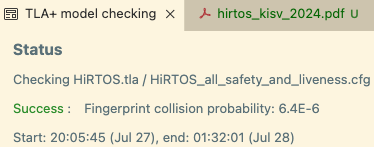
\includegraphics{tlc_run.png}}
   \end{center}
   %\caption{TLC run}
   \label{tlcRun}
%\end{figure}

Below are some of the HiRTOS correctness properties that were
verified:

\paragraph{Safety Invariant1:} Once the thread scheduler 
is started, only one thread ca nbe in the ``Running'' state:
\begin{tla}
 HiRTOS.Interrupts_Enabled =>
  IF HiRTOS.Current_Thread_Id /= "Invalid_Thread_Id"
  THEN
     /\ Cardinality(
         {t \in Threads : 
          Thread_Objects[t].State = "Running"}) = 1
     /\ HiRTOS.Current_Thread_Id =
         CHOOSE t \in Threads : 
            Thread_Objects[t].State = "Running"
  ELSE
     {t \in Threads : 
      Thread_Objects[t].State = "Running"} = {}
\end{tla}
\begin{tlatex}
\@x{\@s{4.1} HiRTOS . Interrupts\_Enabled \.{\implies}}%
 \@x{\@s{8.2} {\IF} HiRTOS . Current\_Thread\_Id
 \.{\neq}\@w{Invalid\_Thread\_Id}}%
\@x{\@s{8.2} \.{\THEN}}%
\@x{\@s{20.5} \.{\land} Cardinality (}%
\@x{\@s{35.58} \{ t \.{\in} Threads \.{:}}%
\@x{\@s{40.19} Thread\_Objects [ t ] . State \.{=}\@w{Running} \} ) \.{=} 1}%
\@x{\@s{20.5} \.{\land} HiRTOS . Current\_Thread\_Id \.{=}}%
\@x{\@s{35.58} {\CHOOSE} t \.{\in} Threads \.{:}}%
\@x{\@s{47.88} Thread\_Objects [ t ] . State \.{=}\@w{Running}}%
\@x{\@s{8.2} \.{\ELSE}}%
\@x{\@s{20.5} \{ t \.{\in} Threads \.{:}}%
 \@x{\@s{25.10} Thread\_Objects [ t ] . State \.{=}\@w{Running} \} \.{=} \{
 \}}%
\end{tlatex}

\paragraph{Safety Invariant 2} The thread owning a mutex can never have lower
priority than any thread waiting for the mutex:
\begin{tla}
(HiRTOS.Interrupts_Enabled /\
 HiRTOS.Current_Thread_Id /= "Invalid_Thread_Id") =>
\A m \in Mutexes :
   LET
     t == Mutex_Objects[m].Owner_Thread_Id
     prio_queue == 
       Mutex_Objects[m].Waiting_Threads_Queue
   IN
     (t /= "Invalid_Thread_Id" /\
      ~Is_Thread_Priority_Queue_Empty(
         prio_queue)) =>
         \A wt \in UNION { Range(q) :
                           q \in Range(prio_queue) } :
         Thread_Objects[wt].State = 
            "Blocked_On_Mutex" /\
         Thread_Objects[t].Current_Priority >= 
            Thread_Objects[wt].Current_Priority
\end{tla}
\begin{tlatex}
\@x{ ( HiRTOS . Interrupts\_Enabled \.{\land}}%
 \@x{\@s{4.23} HiRTOS . Current\_Thread\_Id \.{\neq}\@w{Invalid\_Thread\_Id} )
 \.{\implies}}%
\@x{ \A\, m \.{\in} Mutexes \.{:}}%
\@x{\@s{7.13} \.{\LET}}%
\@x{\@s{15.33} t \.{\defeq} Mutex\_Objects [ m ] . Owner\_Thread\_Id}%
\@x{\@s{15.33} prio\_queue \.{\defeq}}%
\@x{\@s{23.53} Mutex\_Objects [ m ] . Waiting\_Threads\_Queue}%
\@x{\@s{7.13} \.{\IN}}%
\@x{\@s{15.33} ( t \.{\neq}\@w{Invalid\_Thread\_Id} \.{\land}}%
\@x{\@s{19.56} {\lnot} Is\_Thread\_Priority\_Queue\_Empty (}%
\@x{\@s{34.16} prio\_queue ) ) \.{\implies}}%
\@x{\@s{34.16} \A\, wt \.{\in} {\UNION} \{ Range ( q ) \.{:}}%
\@x{\@s{97.34} q \.{\in} Range ( prio\_queue ) \} \.{:}}%
\@x{\@s{34.16} Thread\_Objects [ wt ] . State \.{=}}%
\@x{\@s{46.46}\@w{Blocked\_On\_Mutex} \.{\land}}%
\@x{\@s{34.16} Thread\_Objects [ t ] . Current\_Priority \.{\geq}}%
\@x{\@s{46.46} Thread\_Objects [ wt ] . Current\_Priority}%
\end{tlatex}

\paragraph{Safety Invariant 3}  A thread not owning any mutex and
not waiting on a condvar or  mutex always has its current priority
set to its base priority:

\begin{tla}
HiRTOS.Interrupts_Enabled =>
  \A t \in Threads :
     (Thread_Objects[t].Owned_Mutexes = <<>> /\
      Thread_Objects[t].State \notin 
         {"Blocked_On_Condvar", 
          "Blocked_On_Mutex"}) =>
     Thread_Objects[t].Current_Priority = 
         Thread_Objects[t].Base_Priority
\end{tla}
\begin{tlatex}
\@x{ HiRTOS . Interrupts\_Enabled \.{\implies}}%
\@x{\@s{8.2} \A\, t \.{\in} Threads \.{:}}%
 \@x{\@s{15.33} ( Thread\_Objects [ t ] . Owned\_Mutexes \.{=} {\langle}
 {\rangle} \.{\land}}%
\@x{\@s{19.56} Thread\_Objects [ t ] . State \.{\notin}}%
\@x{\@s{31.86} \{\@w{Blocked\_On\_Condvar} ,\,}%
\@x{\@s{36.47}\@w{Blocked\_On\_Mutex} \} ) \.{\implies}}%
\@x{\@s{15.33} Thread\_Objects [ t ] . Current\_Priority \.{=}}%
\@x{\@s{31.73} Thread\_Objects [ t ] . Base\_Priority}%
\end{tlatex}

\paragraph{Liveness Property 1} Interrupts are not disabled indefinitely:
\begin{tla}
~HiRTOS.Interrupts_Enabled => 
   <>HiRTOS.Interrupts_Enabled
\end{tla}
\begin{tlatex}
\@x{ {\lnot} HiRTOS . Interrupts\_Enabled \.{\implies}}%
\@x{\@s{14.6} {\Diamond} HiRTOS . Interrupts\_Enabled}%
\end{tlatex}


\paragraph{Liveness Property 2} All runnable app threads of the same
priority eventually get the CPU:
\begin{tla}
\A t \in Threads \ { "Idle_Thread" }, 
   p \in Valid_Thread_Priority_Type \ { 0 } :
   (Thread_Objects[t].Current_Priority = p /\ 
    Thread_Objects[t].State = "Runnable") =>
      <>(Thread_Objects[t].State = "Running")
\end{tla}
\begin{tlatex}
 \@x{ \A\, t\@s{1.47} \.{\in} Threads \.{\,\backslash\,} \{\@w{Idle\_Thread}
 \} ,\,}%
 \@x{\@s{7.13} p \.{\in} Valid\_Thread\_Priority\_Type \.{\,\backslash\,} \{ 0
 \} \.{:}}%
\@x{\@s{7.13} ( Thread\_Objects [ t ] . Current\_Priority \.{=} p \.{\land}}%
 \@x{\@s{11.36} Thread\_Objects [ t ] . State \.{=}\@w{Runnable} )
 \.{\implies}}%
 \@x{\@s{19.56} {\Diamond} ( Thread\_Objects [ t ] . State \.{=}\@w{Running}
 )}%
\end{tlatex}

%%
%% The next two lines define the bibliography style to be used, and
%% the bibliography file.
\bibliographystyle{ACM-Reference-Format}
\bibliography{hirtos}

%%
%% If your work has an appendix, this is the place to put it.
%\appendix

\end{document}
\endinput
%%
%% End of file `sample-acmsmall-submission.tex'.
